\documentclass{standalone}
\usepackage{tikz}
\usetikzlibrary{patterns, positioning}

\begin{document}
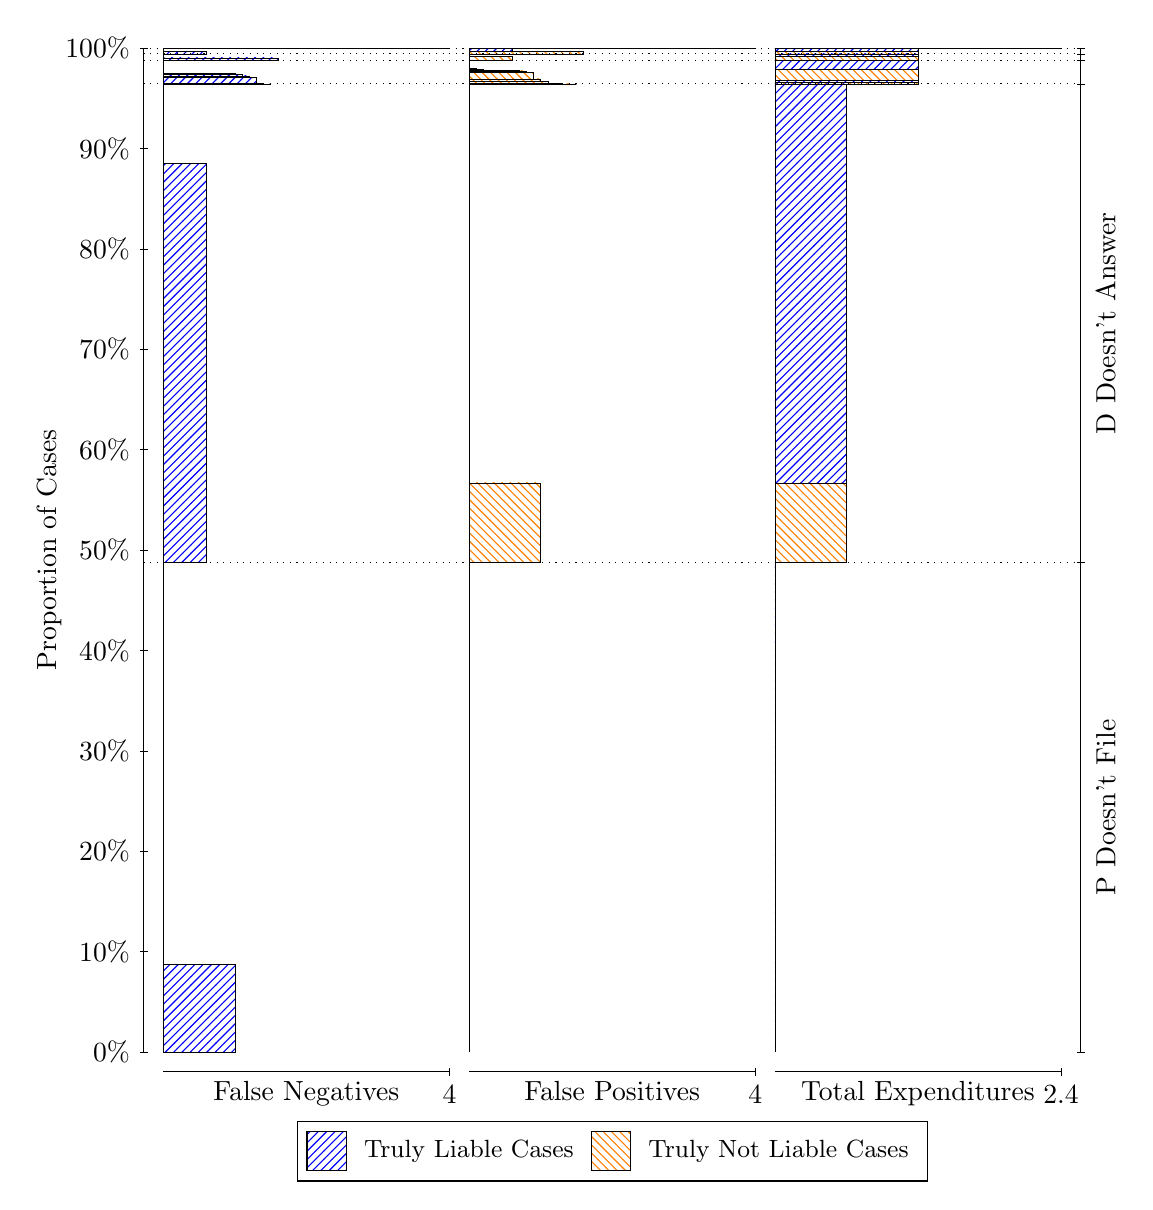
\begin{tikzpicture}
\draw[black, very thin] (1.5,1.75) -- (1.5,14.5);
\node[rotate=90, anchor=center] at (0.3, 8.125) {Proportion of Cases};
\draw[black, very thin] (1.45,1.75) -- (1.55,1.75);
\node[anchor=east] at (1.45, 1.75) {0\%};
\draw[black, very thin] (1.45,3.025) -- (1.55,3.025);
\node[anchor=east] at (1.45, 3.025) {10\%};
\draw[black, very thin] (1.45,4.3) -- (1.55,4.3);
\node[anchor=east] at (1.45, 4.3) {20\%};
\draw[black, very thin] (1.45,5.575) -- (1.55,5.575);
\node[anchor=east] at (1.45, 5.575) {30\%};
\draw[black, very thin] (1.45,6.85) -- (1.55,6.85);
\node[anchor=east] at (1.45, 6.85) {40\%};
\draw[black, very thin] (1.45,8.125) -- (1.55,8.125);
\node[anchor=east] at (1.45, 8.125) {50\%};
\draw[black, very thin] (1.45,9.4) -- (1.55,9.4);
\node[anchor=east] at (1.45, 9.4) {60\%};
\draw[black, very thin] (1.45,10.675) -- (1.55,10.675);
\node[anchor=east] at (1.45, 10.675) {70\%};
\draw[black, very thin] (1.45,11.95) -- (1.55,11.95);
\node[anchor=east] at (1.45, 11.95) {80\%};
\draw[black, very thin] (1.45,13.225) -- (1.55,13.225);
\node[anchor=east] at (1.45, 13.225) {90\%};
\draw[black, very thin] (1.45,14.5) -- (1.55,14.5);
\node[anchor=east] at (1.45, 14.5) {100\%};

\draw[black, very thin] (13.4,1.75) -- (13.4,14.5);
\draw[black, very thin] (13.35,1.75) -- (13.45,1.75);
\node[anchor=west] at (13.35, 1.75) {};
\draw[black, very thin] (13.35,7.9655) -- (13.45,7.9655);
\node[anchor=west] at (13.35, 7.9655) {};
\draw[black, very thin] (13.35,14.044) -- (13.45,14.044);
\node[anchor=west] at (13.35, 14.044) {};
\draw[black, very thin] (13.35,14.346) -- (13.45,14.346);
\node[anchor=west] at (13.35, 14.346) {};
\draw[black, very thin] (13.35,14.426) -- (13.45,14.426);
\node[anchor=west] at (13.35, 14.426) {};
\draw[black, very thin] (13.35,14.494) -- (13.45,14.494);
\node[anchor=west] at (13.35, 14.494) {};
\draw[black, very thin] (13.35,14.498) -- (13.45,14.498);
\node[anchor=west] at (13.35, 14.498) {};
\draw[black, very thin] (13.35,14.5) -- (13.45,14.5);
\node[anchor=west] at (13.35, 14.5) {};

\draw[black, very thin, pattern color=blue, pattern=north east lines] (1.75,1.75) rectangle (2.6583,2.8605);
\draw[black, very thin, pattern color=orange, pattern=north west lines] (1.75,2.8605) rectangle (1.75,7.9655);
\draw[black, very thin, pattern color=blue, pattern=north east lines] (1.75,7.9655) rectangle (2.295,13.032);
\draw[black, very thin, pattern color=orange, pattern=north west lines] (1.75,13.032) rectangle (1.75,14.044);
\draw[black, very thin, pattern color=blue, pattern=north east lines] (1.75,14.044) rectangle (3.1125,14.045);
\draw[black, very thin, pattern color=blue, pattern=north east lines] (1.75,14.045) rectangle (3.0217,14.054);
\draw[black, very thin, pattern color=blue, pattern=north east lines] (1.75,14.054) rectangle (2.9308,14.124);
\draw[black, very thin, pattern color=blue, pattern=north east lines] (1.75,14.124) rectangle (2.84,14.146);
\draw[black, very thin, pattern color=blue, pattern=north east lines] (1.75,14.146) rectangle (2.7492,14.164);
\draw[black, very thin, pattern color=blue, pattern=north east lines] (1.75,14.164) rectangle (2.6583,14.173);
\draw[black, very thin, pattern color=blue, pattern=north east lines] (1.75,14.173) rectangle (2.5675,14.177);
\draw[black, very thin, pattern color=blue, pattern=north east lines] (1.75,14.177) rectangle (2.4767,14.177);
\draw[black, very thin, pattern color=blue, pattern=north east lines] (1.75,14.177) rectangle (2.3858,14.177);
\draw[black, very thin, pattern color=orange, pattern=north west lines] (1.75,14.177) rectangle (1.75,14.346);
\draw[black, very thin, pattern color=blue, pattern=north east lines] (1.75,14.346) rectangle (3.2033,14.375);
\draw[black, very thin, pattern color=orange, pattern=north west lines] (1.75,14.375) rectangle (1.75,14.426);
\draw[black, very thin, pattern color=blue, pattern=north east lines] (1.75,14.426) rectangle (2.295,14.459);
\draw[black, very thin, pattern color=orange, pattern=north west lines] (1.75,14.459) rectangle (1.75,14.494);
\draw[black, very thin, pattern color=blue, pattern=north east lines] (1.75,14.494) rectangle (5.3833,14.495);
\draw[black, very thin, pattern color=orange, pattern=north west lines] (1.75,14.495) rectangle (1.75,14.498);
\draw[black, very thin, pattern color=orange, pattern=north west lines] (1.75,14.498) rectangle (1.75,14.499);
\draw[black, very thin, pattern color=blue, pattern=north east lines] (1.75,14.499) rectangle (1.75,14.5);
\draw[black, very thin, pattern color=orange, pattern=north west lines] (5.6333,1.75) rectangle (5.6333,6.855);
\draw[black, very thin, pattern color=blue, pattern=north east lines] (5.6333,6.855) rectangle (5.6333,7.9655);
\draw[black, very thin, pattern color=orange, pattern=north west lines] (5.6333,7.9655) rectangle (6.5417,8.9771);
\draw[black, very thin, pattern color=blue, pattern=north east lines] (5.6333,8.9771) rectangle (5.6333,14.044);
\draw[black, very thin, pattern color=orange, pattern=north west lines] (5.6333,14.044) rectangle (6.9958,14.044);
\draw[black, very thin, pattern color=orange, pattern=north west lines] (5.6333,14.044) rectangle (6.905,14.044);
\draw[black, very thin, pattern color=orange, pattern=north west lines] (5.6333,14.044) rectangle (6.8142,14.047);
\draw[black, very thin, pattern color=orange, pattern=north west lines] (5.6333,14.047) rectangle (6.7233,14.053);
\draw[black, very thin, pattern color=orange, pattern=north west lines] (5.6333,14.053) rectangle (6.6325,14.076);
\draw[black, very thin, pattern color=orange, pattern=north west lines] (5.6333,14.076) rectangle (6.5417,14.109);
\draw[black, very thin, pattern color=orange, pattern=north west lines] (5.6333,14.109) rectangle (6.4508,14.195);
\draw[black, very thin, pattern color=orange, pattern=north west lines] (5.6333,14.195) rectangle (6.36,14.209);
\draw[black, very thin, pattern color=orange, pattern=north west lines] (5.6333,14.209) rectangle (6.2692,14.213);
\draw[black, very thin, pattern color=blue, pattern=north east lines] (5.6333,14.213) rectangle (6.0875,14.213);
\draw[black, very thin, pattern color=blue, pattern=north east lines] (5.6333,14.213) rectangle (5.9967,14.213);
\draw[black, very thin, pattern color=blue, pattern=north east lines] (5.6333,14.213) rectangle (5.9058,14.217);
\draw[black, very thin, pattern color=blue, pattern=north east lines] (5.6333,14.217) rectangle (5.815,14.226);
\draw[black, very thin, pattern color=blue, pattern=north east lines] (5.6333,14.226) rectangle (5.7242,14.244);
\draw[black, very thin, pattern color=blue, pattern=north east lines] (5.6333,14.244) rectangle (5.6333,14.346);
\draw[black, very thin, pattern color=orange, pattern=north west lines] (5.6333,14.346) rectangle (6.1783,14.396);
\draw[black, very thin, pattern color=blue, pattern=north east lines] (5.6333,14.396) rectangle (5.6333,14.426);
\draw[black, very thin, pattern color=orange, pattern=north west lines] (5.6333,14.426) rectangle (7.0867,14.461);
\draw[black, very thin, pattern color=blue, pattern=north east lines] (5.6333,14.461) rectangle (6.1783,14.494);
\draw[black, very thin, pattern color=orange, pattern=north west lines] (5.6333,14.494) rectangle (5.6333,14.498);
\draw[black, very thin, pattern color=blue, pattern=north east lines] (5.6333,14.498) rectangle (5.6333,14.498);
\draw[black, very thin, pattern color=orange, pattern=north west lines] (5.6333,14.498) rectangle (9.2667,14.499);
\draw[black, very thin, pattern color=blue, pattern=north east lines] (5.6333,14.499) rectangle (8.3583,14.5);
\draw[black, very thin, pattern color=orange, pattern=north west lines] (9.5167,1.75) rectangle (9.5167,6.855);
\draw[black, very thin, pattern color=blue, pattern=north east lines] (9.5167,6.855) rectangle (9.5167,7.9655);
\draw[black, very thin, pattern color=orange, pattern=north west lines] (9.5167,7.9655) rectangle (10.425,8.9771);
\draw[black, very thin, pattern color=blue, pattern=north east lines] (9.5167,8.9771) rectangle (10.425,14.044);
\draw[black, very thin, pattern color=orange, pattern=north west lines] (9.5167,14.044) rectangle (11.333,14.067);
\draw[black, very thin, pattern color=blue, pattern=north east lines] (9.5167,14.067) rectangle (11.333,14.086);
\draw[black, very thin, pattern color=orange, pattern=north west lines] (9.5167,14.086) rectangle (11.333,14.229);
\draw[black, very thin, pattern color=blue, pattern=north east lines] (9.5167,14.229) rectangle (11.333,14.34);
\draw[black, very thin, pattern color=orange, pattern=north west lines] (9.5167,14.34) rectangle (11.333,14.342);
\draw[black, very thin, pattern color=blue, pattern=north east lines] (9.5167,14.342) rectangle (11.333,14.346);
\draw[black, very thin, pattern color=orange, pattern=north west lines] (9.5167,14.346) rectangle (11.333,14.396);
\draw[black, very thin, pattern color=blue, pattern=north east lines] (9.5167,14.396) rectangle (11.333,14.426);
\draw[black, very thin, pattern color=orange, pattern=north west lines] (9.5167,14.426) rectangle (11.333,14.461);
\draw[black, very thin, pattern color=blue, pattern=north east lines] (9.5167,14.461) rectangle (11.333,14.494);
\draw[black, very thin, pattern color=orange, pattern=north west lines] (9.5167,14.494) rectangle (13.15,14.498);
\draw[black, very thin, pattern color=blue, pattern=north east lines] (9.5167,14.498) rectangle (13.15,14.498);
\draw[black, very thin, pattern color=orange, pattern=north west lines] (9.5167,14.498) rectangle (13.15,14.499);
\draw[black, very thin, pattern color=blue, pattern=north east lines] (9.5167,14.499) rectangle (13.15,14.5);
\draw[black, dotted] (1.5,7.9655) -- (13.4,7.9655);
\draw[black, dotted] (1.5,14.044) -- (13.4,14.044);
\draw[black, dotted] (1.5,14.346) -- (13.4,14.346);
\draw[black, dotted] (1.5,14.426) -- (13.4,14.426);
\draw[black, dotted] (1.5,14.494) -- (13.4,14.494);
\draw[black, dotted] (1.5,14.498) -- (13.4,14.498);
\draw[black, very thin] (1.75,1.5) -- (5.3833,1.5);
\node[anchor=north] at (3.5667, 1.5) {False Negatives};
\draw[black, very thin] (5.3833,1.45) -- (5.3833,1.55);
\node[anchor=north] at (5.3833, 1.45) {4};

\draw[black, very thin] (5.6333,1.5) -- (9.2667,1.5);
\node[anchor=north] at (7.45, 1.5) {False Positives};
\draw[black, very thin] (9.2667,1.45) -- (9.2667,1.55);
\node[anchor=north] at (9.2667, 1.45) {4};

\draw[black, very thin] (9.5167,1.5) -- (13.15,1.5);
\node[anchor=north] at (11.333, 1.5) {Total Expenditures};
\draw[black, very thin] (13.15,1.45) -- (13.15,1.55);
\node[anchor=north] at (13.15, 1.45) {2.4};

\node[black, centered, rotate=90] at (13.72, 4.8577) {P Doesn't File};
\node[black, centered, rotate=90] at (13.72, 11.005) {D Doesn't Answer};






\draw (7.449999999999999,1.5) node[draw=none] (baseCoordinate) {};
\begin{scope}[align=center]
        \matrix[scale=0.5, draw=black, below=0.5cm of baseCoordinate, nodes={draw}, column sep=0.1cm]{
            \node[rectangle, draw, minimum width=0.5cm, minimum height=0.5cm, pattern=north east lines, pattern color=blue] {}; &
            \node[draw=none, font=\small] (B) {Truly Liable Cases}; &
            \node[rectangle, draw, minimum width=0.5cm, minimum height=0.5cm, pattern=north west lines, pattern color=orange] {}; &
            \node[draw=none, font=\small] (B) {Truly Not Liable Cases}; \\
            };
\end{scope}

\end{tikzpicture}
\end{document}